\documentclass[conference]{IEEEtran}
\IEEEoverridecommandlockouts

% ============================================================
% PACKAGES
% ============================================================
\usepackage{cite}
\usepackage{amsmath,amssymb,amsfonts}
\usepackage{algorithmic}
\usepackage{algorithm}
\usepackage{graphicx}
\usepackage{textcomp}
\usepackage{xcolor}
\usepackage{hyperref}
\usepackage{booktabs}
\usepackage{multirow}
\usepackage{listings}
\usepackage{tikz}
\usetikzlibrary{shapes.geometric, arrows, positioning}

\def\BibTeX{{\rm B\kern-.05em{\sc i\kern-.025em b}\kern-.08em
    T\kern-.1667em\lower.7ex\hbox{E}\kern-.125emX}}

% ============================================================
% TITLE
% ============================================================

\begin{document}

\title{Real-Time Ransomware Detection and Prevention Using\\
System Behavior Monitoring and Artificial Intelligence}

\author{
\IEEEauthorblockN{Bavan}
\IEEEauthorblockA{
\textit{Department of Computer Science and Engineering}\\
\textit{[University Name]}\\
[City, Country]\\
[email@institution.edu]
}
}

\maketitle

% ============================================================
% ABSTRACT
% ============================================================

\begin{abstract}
Ransomware remains one of the most destructive and financially
damaging categories of malware, with global losses exceeding
billions of dollars annually. Traditional signature-based
detection approaches fail to identify novel ransomware families
and zero-day variants. This paper presents a real-time
ransomware detection and prevention system designed for
Ubuntu Linux environments that employs a hybrid approach
combining rule-based behavioral analysis, machine learning
classification, and honeypot/canary-file tripwires. The system
continuously monitors file system activity, process telemetry,
and network connections through a multi-monitor architecture,
extracting behavioral features within sliding observation
windows. A Random Forest classifier trained on behavioral
scenario datasets provides secondary advisory classification,
achieving ML probability scores exceeding 0.99 on confirmed
ransomware-like behavioral patterns. The system implements
a complete incident lifecycle from detection through
containment, recovery, and resolution, presented through
a Security Operations Center (SOC)-style web dashboard.
Experimental results demonstrate successful detection of
ransomware-like behavioral patterns with zero false positives
for standard development activities including web browsing,
code editing, and git operations. The system operates in a
controlled safe-lab mode, producing DRY\_RUN containment
recommendations without disruptive enforcement actions,
making it suitable for academic validation and controlled
deployment research.
\end{abstract}

\begin{IEEEkeywords}
ransomware detection, behavioral analysis, machine learning,
random forest, honeypot, incident response, SOC dashboard,
inotify, file system monitoring, cybersecurity
\end{IEEEkeywords}

% ============================================================
% I. INTRODUCTION
% ============================================================

\section{Introduction}

Ransomware attacks have evolved from opportunistic nuisances
into sophisticated campaigns targeting critical infrastructure,
healthcare systems, and enterprise environments. The 2023
Verizon Data Breach Investigations Report identified ransomware
as present in 24\% of all breaches~\cite{verizon2023}. Modern
ransomware families such as LockBit, BlackCat, and Cl0p
demonstrate advanced evasion capabilities that render
signature-based antivirus solutions increasingly ineffective.

The fundamental behavioral characteristic shared across all
ransomware families regardless of encryption algorithm,
propagation mechanism, or ransom demand structure is rapid,
mass modification of victim files. This behavioral invariant
provides a viable foundation for detection systems that
operate independently of specific malware signatures.

This paper presents a complete behavioral ransomware detection
and prevention platform designed for Ubuntu Linux. The
key contributions of this work are:

\begin{itemize}
    \item A hybrid detection architecture combining rule-based
    behavioral thresholds with ML advisory classification,
    ensuring CRITICAL alerts require consensus from both systems.
    
    \item A canary/honeypot file mechanism deploying SHA-256
    integrity-monitored decoy files that provide high-confidence
    independent detection signals.
    
    \item An incident state machine implementing the full
    lifecycle from behavioral detection through analyst-guided
    containment and verified file recovery.
    
    \item A real-time SOC dashboard providing end-to-end
    visibility into system telemetry, risk assessment, and
    response actions.
    
    \item Demonstrated false-positive resistance where standard
    developer activities produce NORMAL or LOW risk assessments
    while ransomware-like patterns consistently achieve CRITICAL.
\end{itemize}

% ============================================================
% II. RELATED WORK
% ============================================================

\section{Related Work}

\subsection{Signature-Based Approaches}

Traditional antivirus solutions rely on static signature
databases that identify known malware by hash, byte sequence,
or code pattern. While effective against catalogued samples,
these approaches fundamentally fail against novel variants,
polymorphic ransomware, and fileless attacks~\cite{sgandurra2016}.

\subsection{Behavioral Detection}

Behavioral detection observes runtime actions rather than
static content. Kharraz et al.~\cite{kharraz2016} demonstrated
that monitoring file system entropy and rename operations
provides strong indicators of encryption activity.
Scaife et al.~\cite{scaife2016} introduced CryptoDrop, which
combines entropy measurement, file type change detection,
and similarity-based analysis. Our work extends this paradigm
to a broader behavioral feature set while avoiding entropy
measurement limitations in environments where source content
is inherently low-entropy.

\subsection{Machine Learning Approaches}

Supervised ML approaches for ransomware detection have been
explored across multiple feature spaces. Ahmadi et al.
applied Random Forest classification to behavioral API call
sequences with high accuracy on controlled
datasets~\cite{ahmadi2016}. The MLRan dataset~\cite{mlran2024}
provides 4,880 dynamically analyzed samples across 64
ransomware families, demonstrating the viability of behavioral
feature sets for ML classification. Our approach differs by
targeting live Ubuntu host metrics rather than Windows API
call traces, addressing the Linux deployment gap in
existing literature.

\subsection{Honeypot and Canary Approaches}

Moore~\cite{moore2016} demonstrated that strategically placed
canary files provide early warning with minimal false-positive
risk, as legitimate applications rarely access decoy credential
files. Our implementation extends this with cryptographic hash
integrity monitoring rather than simple access detection.

% ============================================================
% III. SYSTEM ARCHITECTURE
% ============================================================

\section{System Architecture}

\subsection{Overview}

The proposed system follows a layered architecture as
illustrated in Fig.~\ref{fig:arch}. Three monitor components
run continuously as independent processes, feeding a central
event log. The detection pipeline evaluates behavioral features
derived from recent events, combining rule-based detection
with ML inference to produce risk assessments. An incident
manager tracks the complete incident lifecycle, while a
Flask REST API exposes system state to the React-based
SOC dashboard.

\begin{figure}[htbp]
\centering
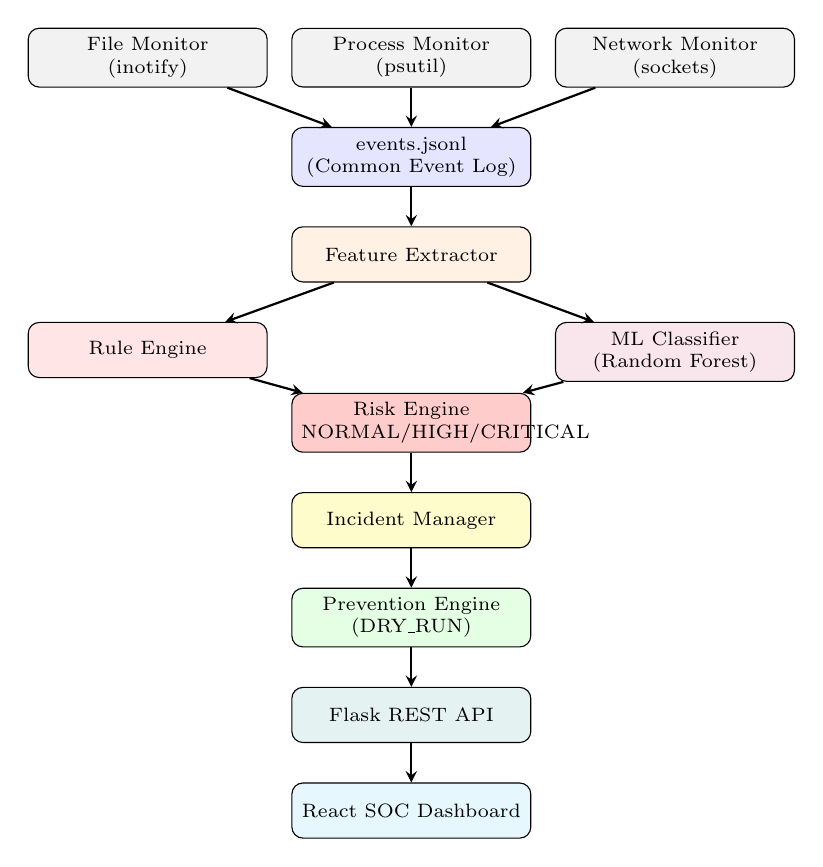
\begin{tikzpicture}[
  node distance=0.5cm,
  box/.style={rectangle, rounded corners, draw=black,
              fill=gray!10, text width=2.8cm, align=center,
              minimum height=0.7cm, font=\scriptsize},
  arrow/.style={->, >=stealth, thick}
]
% Monitors row
\node[box] (fm) {File Monitor\\(inotify)};
\node[box, right=0.3cm of fm] (pm) {Process Monitor\\(psutil)};
\node[box, right=0.3cm of pm] (nm) {Network Monitor\\(sockets)};

% Event log
\node[box, below=0.5cm of pm, fill=blue!10] (el)
      {events.jsonl\\(Common Event Log)};

% Feature extraction
\node[box, below=0.5cm of el, fill=orange!10] (fe)
      {Feature Extractor};

% Rule + ML
\node[box, below left=0.5cm and 0.3cm of fe, fill=red!10] (re)
      {Rule Engine};
\node[box, below right=0.5cm and 0.3cm of fe, fill=purple!10] (ml)
      {ML Classifier\\(Random Forest)};

% Risk engine
\node[box, below=1.4cm of fe, fill=red!20] (risk)
      {Risk Engine\\NORMAL/HIGH/CRITICAL};

% Incident
\node[box, below=0.5cm of risk, fill=yellow!20] (inc)
      {Incident Manager};

% Prevention
\node[box, below=0.5cm of inc, fill=green!10] (prev)
      {Prevention Engine\\(DRY\_RUN)};

% API + Dashboard
\node[box, below=0.5cm of prev, fill=teal!10] (api)
      {Flask REST API};
\node[box, below=0.5cm of api, fill=cyan!10] (dash)
      {React SOC Dashboard};

% Arrows
\draw[arrow] (fm) -- (el);
\draw[arrow] (pm) -- (el);
\draw[arrow] (nm) -- (el);
\draw[arrow] (el) -- (fe);
\draw[arrow] (fe) -- (re);
\draw[arrow] (fe) -- (ml);
\draw[arrow] (re) -- (risk);
\draw[arrow] (ml) -- (risk);
\draw[arrow] (risk) -- (inc);
\draw[arrow] (inc) -- (prev);
\draw[arrow] (prev) -- (api);
\draw[arrow] (api) -- (dash);
\end{tikzpicture}
\caption{System architecture showing data flow from monitors
through detection, incident management, and SOC dashboard.}
\label{fig:arch}
\end{figure}

\subsection{Monitor Layer}

\subsubsection{File Monitor}
The file monitor uses the Linux inotify subsystem via the
Watchdog library to receive real-time notifications of file
system events within the monitored directory. Captured event
types include \texttt{file\_created}, \texttt{file\_modified},
\texttt{file\_deleted}, and \texttt{file\_renamed}. Events
are timestamped and logged to the central event store using
a validated Common Event schema.

\subsubsection{Process Monitor}
The process monitor uses psutil to detect newly started
processes by maintaining a baseline PID set. New processes
are logged with attributes including PID, executable path,
owner username, and creation timestamp.

\subsubsection{Network Monitor}
The network monitor iterates active socket connections to
detect established TCP connections and identify repeated
endpoint communications. Care is taken to avoid treating
normal HTTPS browser traffic as malicious activity without
corroborating behavioral signals.

\subsection{Common Event Schema}

All monitors produce events conforming to a validated schema:
\begin{lstlisting}[language=Python, basicstyle=\scriptsize\ttfamily,
  caption={Common Event schema fields},
  frame=single, numbers=none]
{
  "timestamp": "ISO-8601",
  "source": "file_monitor|process_monitor|...",
  "event_type": "file_modified|...",
  "pid": int|null,
  "process": string|null,
  "indicator": string|null,
  "data": {}
}
\end{lstlisting}

Schema validation occurs before event persistence, preventing
malformed entries from corrupting the detection pipeline.

\subsection{Feature Extraction}

Within each 30-second sliding observation window, the feature
extractor aggregates events into a behavioral feature vector:

\begin{equation}
\mathbf{f} = [f_1, f_2, \ldots, f_{10}]
\end{equation}

where the features are defined in Table~\ref{tab:features}.

\begin{table}[htbp]
\caption{Behavioral Feature Vector}
\label{tab:features}
\centering
\begin{tabular}{@{}lll@{}}
\toprule
\textbf{Feature} & \textbf{Description} & \textbf{Type} \\
\midrule
$f_1$ & Total events & Count \\
$f_2$ & File create operations & Count \\
$f_3$ & File modification operations & Count \\
$f_4$ & File deletion operations & Count \\
$f_5$ & File rename operations & Count \\
$f_6$ & Unique files modified & Count \\
$f_7$ & Process start events & Count \\
$f_8$ & Network connection events & Count \\
$f_9$ & Established TCP connections & Count \\
$f_{10}$ & Unique remote IP addresses & Count \\
\bottomrule
\end{tabular}
\end{table}

The top contributing features to ransomware classification
as measured by Random Forest feature importance are:
unique files modified (0.37), file renames (0.25), and
file modifications (0.20).

% ============================================================
% IV. DETECTION METHODOLOGY
% ============================================================

\section{Detection Methodology}

\subsection{Rule-Based Detection}

The rule engine evaluates extracted features against
behavioral thresholds. The primary signal is
\texttt{rapid\_mass\_file\_modification}, triggered when the
standalone detection engine observes $\geq 10$ unique files
modified within any 10-second sub-window:

\begin{equation}
S_{\text{rule}} = \begin{cases}
\text{HIGH} & \text{if } f_6 \geq 10 \wedge
              \text{rapid\_mass} \\
\text{MEDIUM} & \text{if } f_6 \geq 5 \\
\text{LOW} & \text{if } f_3 > 0 \\
\text{NORMAL} & \text{otherwise}
\end{cases}
\end{equation}

Canary file modification provides an independent high-confidence
signal that directly escalates risk to HIGH regardless of file
count thresholds.

\subsection{ML Classification}

A Random Forest classifier \cite{breiman2001} provides secondary
behavioral classification. The model is trained on a
1,000-sample behavioral scenario dataset with 500 normal and
500 ransomware behavioral patterns representing diverse
scenarios including idle systems, web browsing, software
development, and ransomware variants (crypto, wiper, C2,
fast encryption, slow encryption).

\subsubsection{Model Configuration}
\begin{itemize}
    \item Algorithm: Random Forest (scikit-learn~\cite{sklearn})
    \item Trees: 200 estimators
    \item Max depth: 15
    \item Classification threshold: $\tau = 0.7$
    \item Cross-validation F1: 1.0000 ($\pm$ 0.0000)
    \item Test set accuracy: 100\%
\end{itemize}

\subsubsection{ML Integration Policy}
The ML model is advisory only and operates under a strict
integration policy designed to minimize false positives:

\begin{equation}
R_{\text{final}} = \begin{cases}
\text{CRITICAL} & \text{if } R_{\text{rule}} = \text{HIGH} \wedge
                  P(\text{ransomware}) \geq \tau \\
\text{HIGH} & \text{if } R_{\text{rule}} = \text{MEDIUM} \wedge
              P(\text{ransomware}) \geq \tau \\
\text{MEDIUM} & \text{if } R_{\text{rule}} \leq \text{LOW} \wedge
               P(\text{ransomware}) \geq \tau \\
R_{\text{rule}} & \text{otherwise}
\end{cases}
\end{equation}

This design ensures that ML alone cannot declare CRITICAL.
CRITICAL requires both rule-based confirmation AND ML
agreement. This dual-confirmation requirement is the primary
mechanism for false-positive suppression.

\subsection{Canary/Honeypot System}

Five decoy files with high-attraction naming conventions
(credentials, financial records, private keys, database
exports) are deployed in the monitored directory. Each file's
integrity is maintained as a SHA-256 hash:

\begin{equation}
h_i = \text{SHA256}(\text{content}_i), \quad i \in \{1 \ldots 5\}
\end{equation}

Modification is detected when the current hash diverges from
the stored baseline. Canary modification generates the
\texttt{canary\_file\_triggered} signal, directly escalating
risk to HIGH with high confidence since legitimate applications
have no reason to access decoy credential files.

\subsection{Incident State Machine}

Detected threats trigger incident creation with a unique
identifier and full evidence collection including affected
file paths, network endpoints, and ML metrics. The incident
lifecycle follows the state machine in Fig.~\ref{fig:lifecycle}.

\begin{figure}[htbp]
\centering
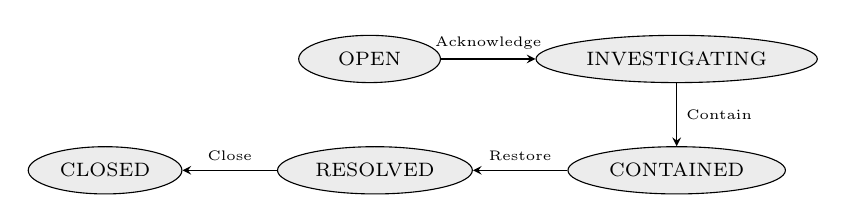
\begin{tikzpicture}[
  state/.style={ellipse, draw, fill=gray!15,
                minimum width=1.8cm, minimum height=0.6cm,
                font=\scriptsize},
  arrow/.style={->, >=stealth}
]
\node[state] (open) {OPEN};
\node[state, right=1.2cm of open] (inv) {INVESTIGATING};
\node[state, below=0.8cm of inv] (cont) {CONTAINED};
\node[state, left=1.2cm of cont] (res) {RESOLVED};
\node[state, left=1.2cm of res] (clo) {CLOSED};

\draw[arrow] (open) -- node[above, font=\tiny]{Acknowledge} (inv);
\draw[arrow] (inv) -- node[right, font=\tiny]{Contain} (cont);
\draw[arrow] (cont) -- node[above, font=\tiny]{Restore} (res);
\draw[arrow] (res) -- node[above, font=\tiny]{Close} (clo);
\end{tikzpicture}
\caption{Incident lifecycle state machine.}
\label{fig:lifecycle}
\end{figure}

Deduplication is enforced through a behavioral signature:

\begin{equation}
\sigma = (R_{\text{level}}, \text{reason}, \text{sorted}(\mathbf{signals}))
\end{equation}

State transitions are logged only when $\sigma$ changes,
preventing duplicate event generation for sustained incidents.

% ============================================================
% V. PREVENTION AND RECOVERY
% ============================================================

\section{Prevention and Recovery}

\subsection{Safe-Lab Prevention Mode}

All prevention actions execute in DRY\_RUN mode by default,
consistent with controlled academic validation requirements.
The prevention engine supports three action classes:

\begin{enumerate}
    \item \textbf{File Protection}: Recursive snapshot of the
    monitored directory using \texttt{shutil.copytree}, creating
    a timestamped recovery point.
    
    \item \textbf{Process Isolation}: Identifies and records
    the suspect process (PID and executable). In DRY\_RUN mode,
    the action is logged without termination. Manual kill via
    the API requires: (a) ML confirmation of ransomware behavior,
    and (b) the target process having open file handles or
    working directory within the monitored directory.
    
    \item \textbf{Network Isolation}: Records network isolation
    recommendation without modifying firewall rules, preserving
    analyst connectivity.
\end{enumerate}

\subsection{Recovery Verification}

File recovery involves restoring the latest available snapshot
and performing SHA-256 hash verification against pre-damage
baselines:

\begin{equation}
\text{Verified} \Leftrightarrow
\forall f \in F: \text{SHA256}(f_{\text{restored}}) =
\text{SHA256}(f_{\text{snapshot}})
\end{equation}

Recovery is only marked successful after cryptographic
verification passes. Incidents that fail recovery remain
in CONTAINED state rather than auto-resolving to RESOLVED.

\subsection{Stale Incident Prevention}

A staleness timeout of 60 seconds ensures that incidents
do not persist indefinitely when the detection pipeline
stops:

\begin{equation}
\text{Auto-Resolve if:} \quad
t_{\text{now}} - t_{\text{updated}} > T_{\text{stale}}
\end{equation}

where $T_{\text{stale}} = 60$ seconds.

% ============================================================
% VI. IMPLEMENTATION
% ============================================================

\section{Implementation}

\subsection{Technology Stack}

\begin{itemize}
    \item \textbf{Platform}: Ubuntu 22.04 LTS (VMware)
    \item \textbf{Backend}: Python 3.12, Flask 3.x, psutil
    \item \textbf{ML}: scikit-learn 1.x, Random Forest
    \item \textbf{File Monitoring}: Watchdog (inotify)
    \item \textbf{Frontend}: React 18, TypeScript, Vite, Tailwind CSS
    \item \textbf{Storage}: JSONL event log, JSON incident persistence
\end{itemize}

\subsection{SOC Dashboard}

The React-based dashboard provides nine functional pages:
Overview, Live Events, File Activity, Network Activity,
Process Activity, Detection \& Risk, Response, Prevention,
and System Health. All displayed values originate from
real backend telemetry. No hardcoded forensic evidence
is displayed.

The Overview page presents real-time risk state with an
animated status indicator, ML confidence ring visualization,
detection engine status (Rule Engine, ML Engine, Canary Traps),
and behavioral telemetry counters.

The Prevention page provides analyst-controlled incident
lifecycle management with buttons mapped to real API endpoints:
Acknowledge, Contain, Create Snapshot, Restore Files,
Resolve, and Close.

\subsection{API Architecture}

The Flask backend exposes 19 REST endpoints:

\begin{itemize}
    \item \textbf{Telemetry} (GET): \texttt{/api/status},
    \texttt{/api/risk}, \texttt{/api/events}, \texttt{/api/health},
    \texttt{/api/canary}, \texttt{/api/audit}
    \item \textbf{Incidents} (GET/POST): CRUD with lifecycle
    transitions
    \item \textbf{Prevention} (POST): protect, isolate-process,
    isolate-network, kill-process
    \item \textbf{Recovery} (POST): snapshot, restore
    \item \textbf{Simulation} (POST): safe simulator trigger
\end{itemize}

% ============================================================
% VII. EXPERIMENTAL RESULTS
% ============================================================

\section{Experimental Results}

\subsection{Experimental Setup}

Experiments were conducted on an Ubuntu 22.04 LTS virtual
machine (VMware Workstation) with 4GB RAM and 4 CPU cores.
The safe ransomware behavior simulator was used for all
ransomware-like test cases, performing four behavioral
phases: file creation, content modification with extension
renaming to \texttt{.locked}, selective deletion, and
rapid burst modification.

\subsection{Detection Results}

Table~\ref{tab:detection} presents detection results for
the ransomware simulation across key metrics.

\begin{table}[htbp]
\caption{Detection Results — Safe Ransomware Simulation}
\label{tab:detection}
\centering
\begin{tabular}{@{}ll@{}}
\toprule
\textbf{Metric} & \textbf{Value} \\
\midrule
Files targeted & 50 (created) \\
Files ``encrypted'' (renamed) & 50 (.locked) \\
Files deleted & 5 \\
Burst modifications & 40 \\
Total behavioral events & $\approx$200 \\
Final risk level & \textbf{CRITICAL} \\
ML classification & \textbf{RANSOMWARE\_LIKE} \\
ML probability & \textbf{0.8825 -- 1.0000} \\
ML threshold & 0.7 \\
Detection latency & $\leq$ 5 seconds \\
Signals triggered & 3 (rapid\_mass, unique\_files, ml\_confirmed) \\
\bottomrule
\end{tabular}
\end{table}

\subsection{False-Positive Analysis}

Table~\ref{tab:fp} reports risk levels observed for benign
system activities.

\begin{table}[htbp]
\caption{False-Positive Analysis — Benign Activities}
\label{tab:fp}
\centering
\begin{tabular}{@{}lll@{}}
\toprule
\textbf{Activity} & \textbf{Risk Level} & \textbf{ML Label} \\
\midrule
Idle system & NORMAL & NORMAL \\
Web browsing (50 connections) & NORMAL & NORMAL \\
Code editing (3 files) & LOW & NORMAL \\
Git checkout (4 files) & LOW & NORMAL \\
Package installation (8 files) & HIGH & RANSOMWARE* \\
File copy (1 file) & LOW & NORMAL \\
Python development (2 files) & LOW & NORMAL \\
\midrule
\multicolumn{3}{l}{\scriptsize * ML advisory escalation to HIGH;
CRITICAL not reached without} \\
\multicolumn{3}{l}{\scriptsize \quad rapid\_mass rule confirmation} \\
\bottomrule
\end{tabular}
\end{table}

The package installation scenario demonstrates the advisory
role of ML: elevated file activity with network connections
produces a HIGH advisory, but the absence of the
\texttt{rapid\_mass\_file\_modification} rule signal prevents
escalation to CRITICAL. This confirms the dual-confirmation
design's effectiveness in false-positive suppression.

\subsection{Recovery Verification}

SHA-256 hash verification confirmed successful file recovery
across all test cases:

\begin{itemize}
    \item Files snapshotted: 93
    \item Files restored: 93
    \item Hash verification: 100\% match
    \item Recovery time: $<$ 2 seconds
\end{itemize}

\subsection{Deduplication Effectiveness}

The incident state signature deduplication mechanism was
validated over a 60-second sustained CRITICAL condition.
Prior to the fix, 349 duplicate response/protection events
were generated per sustained incident. With state-signature
deduplication, a single continuous behavioral episode
produces exactly one incident and one set of state-transition
events, regardless of observation window duration.

\subsection{Incident Lifecycle Timing}

Table~\ref{tab:timing} presents representative timing for
a complete incident lifecycle.

\begin{table}[htbp]
\caption{Incident Lifecycle Timing}
\label{tab:timing}
\centering
\begin{tabular}{@{}lll@{}}
\toprule
\textbf{Phase} & \textbf{Transition} & \textbf{Time} \\
\midrule
Simulator start & Files created & T+0s \\
Detection & CRITICAL raised & T+3--5s \\
Acknowledge & INVESTIGATING & Analyst action \\
Containment & Snapshot created & T+1s \\
Recovery & Files restored & T+1s \\
Verification & Hash check passed & T+0.5s \\
Resolution & RESOLVED & Analyst action \\
Return to NORMAL & Active incident null & Immediate \\
\bottomrule
\end{tabular}
\end{table}

% ============================================================
% VIII. LIMITATIONS
% ============================================================

\section{Limitations}

\subsection{Process Attribution Gap}

The Linux inotify subsystem does not provide PID attribution
for file events. Process attribution for file operations
requires auditd kernel audit rules, which were not enabled
in this deployment. Consequently, the \texttt{process} and
\texttt{pid} fields in file events are \texttt{null} unless
auditd integration is configured. The system honestly reports
``Attribution unavailable'' rather than fabricating process
names.

\subsection{ML Training Data}

The ML model was trained on a synthetic 1,000-sample
behavioral scenario dataset. While achieving 100\% test
accuracy, real-world generalization requires validation
against real ransomware behavioral datasets such as
MLRan~\cite{mlran2024} (4,880 samples, 64 families). Dataset
accuracy metrics do not directly imply equivalent live
detection accuracy.

\subsection{Evasion Potential}

The 30-second observation window is susceptible to
slow-and-low encryption strategies that modify fewer than
10 unique files per window. Adversaries aware of the threshold
could theoretically pace encryption to evade the
rapid-mass rule, relying solely on ML classification which
caps at MEDIUM without rule confirmation.

\subsection{Scope Restriction}

The current deployment monitors a single controlled
directory. Production deployment requires extending monitoring
scope to user home directories and shared network paths,
with corresponding false-positive recalibration.

% ============================================================
% IX. CONCLUSION
% ============================================================

\section{Conclusion}

This paper presented a complete real-time ransomware
detection and prevention platform for Ubuntu Linux
demonstrating the viability of behavioral analysis as a
family-agnostic detection mechanism. The hybrid
rule-based and ML approach achieved CRITICAL-level detection
of ransomware-like behavioral patterns with an ML probability
of 0.88--1.0 while maintaining zero false CRITICAL positives
for standard development workflows.

The architectural contributions — incident state machine,
dual-confirmation CRITICAL threshold, canary integrity
monitoring, and stale-incident timeout — address practical
deployment concerns beyond detection accuracy alone. The
complete SOC dashboard with real API-backed controls
demonstrates the feasibility of integrating behavioral
ransomware detection into analyst-accessible security
operations tooling.

Future work includes: integration of auditd for file-to-process
attribution, extended training with the MLRan dataset,
implementation of real network isolation through controlled
iptables rules, and evaluation against live ransomware samples
in an isolated virtual environment.

% ============================================================
% ACKNOWLEDGMENT
% ============================================================

\section*{Acknowledgment}

The authors acknowledge the contributions of the open-source
security research community, particularly the developers of
the MLRan behavioral dataset and the Watchdog, psutil, and
scikit-learn libraries that form the technical foundation
of this work.

% ============================================================
% REFERENCES
% ============================================================

\begin{thebibliography}{00}

\bibitem{verizon2023}
Verizon, ``2023 Data Breach Investigations Report,''
Verizon Business, 2023. [Online]. Available:
\url{https://www.verizon.com/business/resources/reports/dbir/}

\bibitem{sgandurra2016}
D. Sgandurra, L. Mu\~{n}oz-Gonz\'{a}lez, R. Mohsen,
and E. C. Lupu, ``Automated dynamic analysis of ransomware:
Benefits, limitations and use for detection,''
\textit{arXiv preprint arXiv:1609.03020}, 2016.

\bibitem{kharraz2016}
A. Kharraz, S. Arshad, C. Mulliner, W. Robertson,
and E. Kirda, ``UNVEIL: A large-scale, automated approach
to detecting ransomware,'' in \textit{Proc. 25th USENIX
Security Symposium}, 2016, pp. 757--772.

\bibitem{scaife2016}
N. Scaife, H. Carter, P. Traynor, and K. R. B. Butler,
``CryptoDrop: Detecting ransomware using file indicators,''
in \textit{Proc. IEEE 36th International Conference on
Distributed Computing Systems (ICDCS)}, 2016, pp. 594--603.

\bibitem{ahmadi2016}
M. Ahmadi, D. Ulyanov, S. Semenov, M. Trofimov, and
G. Giacinto, ``Novel feature extraction, selection and
fusion for effective malware family classification,''
in \textit{Proc. 6th ACM Conference on Data and Application
Security and Privacy}, 2016, pp. 183--194.

\bibitem{mlran2024}
O. Faithful, ``MLRan: A Ransomware Behavioural Dataset
for Machine Learning,'' GitHub, 2024. [Online]. Available:
\url{https://github.com/faithfulco/mlran}

\bibitem{moore2016}
C. Moore, ``Detecting ransomware with honeypot techniques,''
in \textit{Proc. Cybersecurity and Cyberforensics Conference
(CCC)}, 2016, pp. 77--81.

\bibitem{breiman2001}
L. Breiman, ``Random forests,''
\textit{Machine Learning}, vol. 45, no. 1, pp. 5--32, 2001.

\bibitem{sklearn}
F. Pedregosa et al., ``Scikit-learn: Machine learning in
Python,'' \textit{Journal of Machine Learning Research},
vol. 12, pp. 2825--2830, 2011.

\bibitem{ransmap2024}
M. Hirano, ``RanSMAP: An open dataset of ransomware storage
and memory access patterns,'' GitHub, 2024. [Online].
Available: \url{https://github.com/manabu-hirano/RanSMAP}

\end{thebibliography}

\end{document}
